\documentclass{article}


\usepackage{arxiv}

\usepackage[utf8]{inputenc} % allow utf-8 input
\usepackage[T1]{fontenc}    % use 8-bit T1 fonts
\usepackage{hyperref}       % hyperlinks
\usepackage{url}            % simple URL typesetting
\usepackage{booktabs}       % professional-quality tables
\usepackage{amsfonts}       % blackboard math symbols
\usepackage{nicefrac}       % compact symbols for 1/2, etc.
\usepackage{microtype}      % microtypography
\usepackage{lipsum}
\usepackage{graphicx}
\graphicspath{ {./images/} }


\title{k-NN Sampling for Visualization of Dynamic Data Using LION-tSNE - analysis}


\author{
 Gędłek Paweł \\
  Wydział Informatyki, Elektroniki i Telekomunikacji\\
  Akademia Górniczo-Hutnicza \\
  Kraków \\
  \texttt{gedlek@student.agh.edu.pl} \\
  \And
Wójtowicz Patryk \\
  Wydział Informatyki, Elektroniki i Telekomunikacji\\
  Akademia Górniczo-Hutnicza \\
  Kraków \\
  \texttt{wojtowicz@student.agh.edu.pl} \\
}


\begin{document}
\maketitle
\begin{abstract}
TODO
\end{abstract}


% keywords can be removed
% keywords{First keyword \and Second keyword \and More}


\section{Struktura raportu}
\label{sec:report_structure}
\paragraph{}
\tableofcontents

\section{Metoda tSNE}
\label{sec:tSNE}
\paragraph{}
\subsection{Czym właściwie jest tSNE?}
Algorytm tSNE(t-Distributed Stochastic Neighbor Embedding) którego
autorami są Laurens van der Maaten oraz Geoffrey Hinton bazuje na
metodzie SNE, której głównym założeniem jest reprezentacja
wielowymiarowych danych w możliwy do zobrazowania dla człowieka dwu lub
trzy-wymiarowej przestrzeni. Osiąga się to poprzez modelowanie wysoko
wymiarowych obiektów poprzez dwu- lub trzy-wymiarowe punkty w taki
sposób, że zbliżone obiekty modelowane są poprzez bliskie sobie punkty, a
oddalone obiekty modelowane są poprzez oddalone od siebie punkty z
duzym prawdopodobienstwem.

\subsection{Algorytm tSNE - podstawy matematyczne}
\begin{itemize}
\item 
Algorytm tSNE konwertuje odległości między parami punktów w
funkcje rozkładu prawdopodobieństwa określająca podobieństwo
pomiędzy parami punktów.
\item 
Rozbieżność między podobieństwem wysoko wymiarowych danych z
nisko-wymiarowymi danymi jest mierzona poprzez dywergencje
Kullbacka-Leiblera i minimalizowana metoda gradientowa
poszukiwania minimum lokalnego
\end{itemize}

Mamy dany zbiór wejściowy $X = {x1, x2...xn}$ gdzie dla każdego $x_i \in R^{D}$
jest D-wymiarowym wektorem. Zbiór ten zostanie przekształcony do
postaci $Y = {y1, y2...yn}$ gdzie każde $y_i \in R^d$ jest d-wymiarowym
wektorem oraz $d << D$ (zazwyczaj d = 2 lub 3). Podobieństwo pomiędzy
para punktów wejściowych xi oraz xj oznaczamy poprzez pj/i , które jest
prawdopodobieństwem wybrania $x_j$ jako sąsiada $x_i$ według funkcji gęstości
prawdopodobieństwa na rozkładzie normalnym gdzie $x_i$ stanowi centrum.
$p_{j|i}$ definiujemy jako:

\begin{equation}
    p_{j|i} = \frac{exp(\frac{-d(x_i, x_j)^2)}{2\sigma_{i}^2})}{\sum_{k \neq i}^{n} exp(\frac{-d(x_i, x_k)^2)}{2\sigma_{i}^2})} \\
    p_{i|i} = 0 \\
    p_{i|j} = \frac{p_{j|i} + p_{i|j}}{2n} 
\end{equation}

gdzie:

$d(x_i, x_j)$ - odległość pomiędzy punktami $x_i$ oraz $x_j$ w oryginalnym wymiarze

$\sigma_i$ - wariancja dla punktu $x_i$

Aby otrzymać zbiór wyjściowy Y, losujemy n punktów w docelowym
wymiarze i dla każdego z nich wyznaczamy podobna funkcje gęstości
prawdopodobieństwa (tym razem jest to rozkład Studenta):

\begin{equation}
   q_{ij} = \frac{(1 + d(y_i, y_j)^2)^{-1}}{\sum_{k \neq l}^{n}((1 + d(y_k, y_l)^2)^{-1})}
\end{equation}

gdzie:

$d(y_i, y_j)$ - odległość pomiędzy punktami yi oraz yj w docelowym wymiarze

W ten sposób otrzymujemy łączone rozkłady gęstości prawdopodobieństwa
P i Q dla wszystkich punktów ze zbiorów odpowiednio X i Y. Podobieństwo
między nimi (a właściwie dowolnymi 2 rozkładami) określa dywergencja
Kullbacka-Leiblera:

\begin{equation}
    C = KLDIV(P || Q) = \sum_i^n\sum_j^n p_{ij}log \frac{p_{ij}}{q_{ij}}
\end{equation}

która staje sie nasza funkcja kosztu, która chcemy zminimalizować, robi sie
to algorytmem spadku po gradiencie (Gradient Descent). Pochodna
cząstkowa C dla $y_i$ to:

\begin{equation}
\frac{\delta C}{\delta y_i} = 4 \sum_i^n (p_{ij} - q_{ij})(y_i - y_j)(1 + d(y_i - y_j)^2)^{-1}
\end{equation}

\subsection{Sposób wyboru wariancji}

Wariancje $\sigma_i$ dla punktu $x_i$ wybiera się na podstawie parametru algorytmu
ustawianego przez użytkownika zwanego Perplexity. Definiujemy:

\begin{equation}
    Perp(i) = 2^{H(P_i)} H(P_i) = \sum_j p_{j|i} log (\frac{1}{p_{j|i}})
\end{equation}

gdzie:

$H(P_i)$ - entropia Shannona dla zmiennej losowej $P_i$

Dla rozkładu normalnego im większa entropia, tym większa wariancja, tym
”grubsze ogony”funkcji dzwonowej, tym większe prawdopodobieństwo
wybrania bardziej odległych sąsiadów punktu $x_i$ . Zazwyczaj dla wszystkich
punktów $Perp(i)$ ustawiane jest na taka sama wartosc $p$. Im mniej
”gesty”jest nasz zbiór danych tym Perp powinno być większe.

\subsection{Workflow metody tSNE}

\begin{figure}[h]
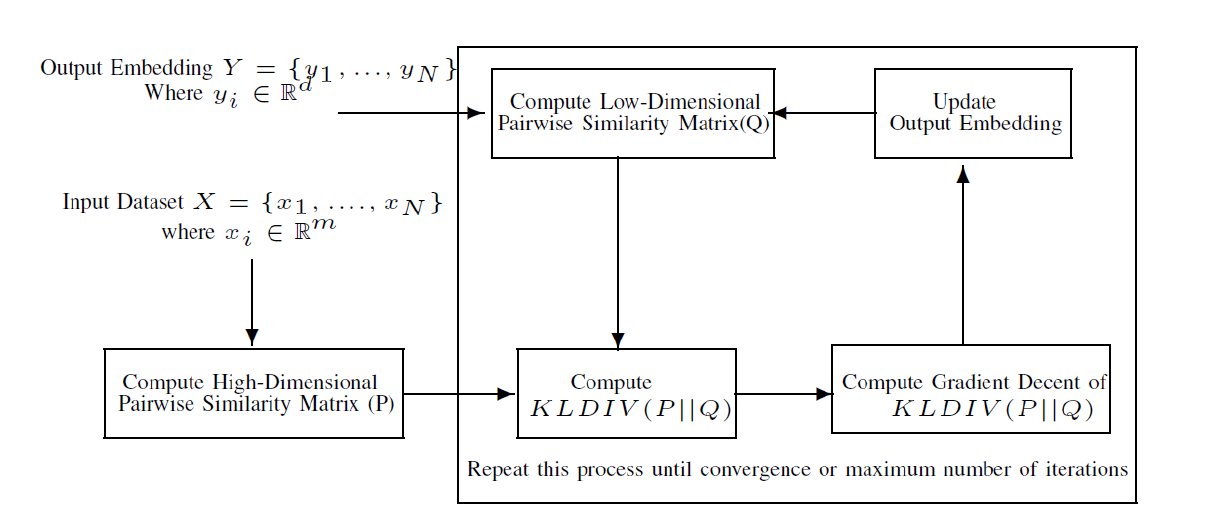
\includegraphics[scale=0.52]{algorithm_TSNE.PNG}
\caption{Algorytm tSNE - workflow modelu}
\end{figure}

\subsection{Pseudokod metody tSNE}

\begin{figure}[h]
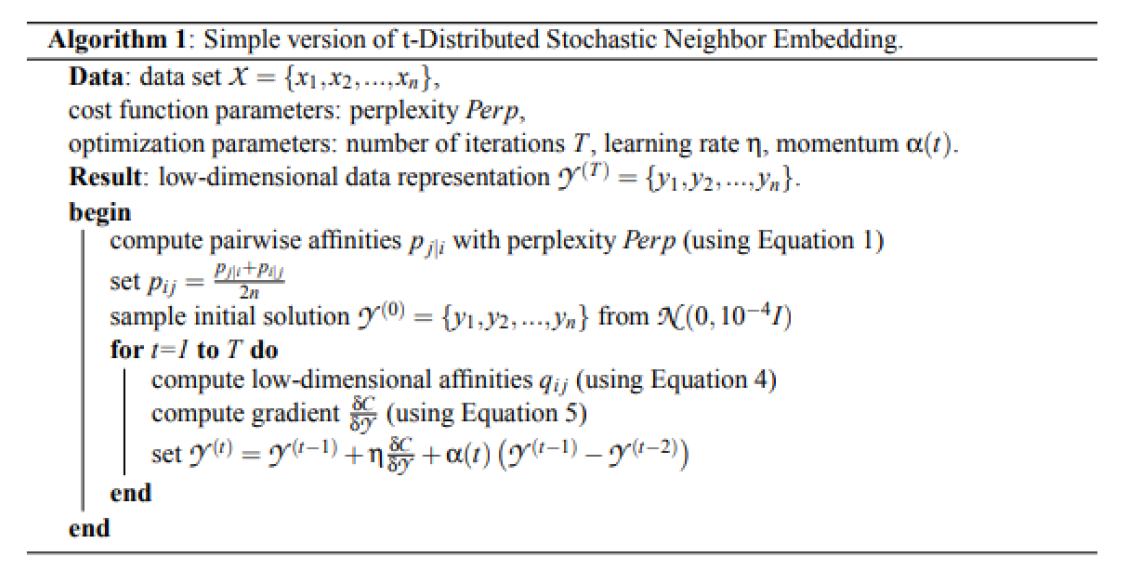
\includegraphics[scale=0.52]{algorithm_TSNE_pseudocode.PNG}
\caption{Algorytm tSNE - pseudokod}
\end{figure}

\section{Metoda LION tSNE}
\label{sec:lionTSNE}
\paragraph{}
Algorytm t-SNE nie odpowiada na pytanie jak dodawać nowe dane (lub
wizualizować dynamiczne zmiany danych) do utworzonego modelu. Z
pomocą przychodzi metoda LION tSNE (Local Interpolation with Outlier
coNtrol t-Distributed Stochastic Neighbor Embedding). Korzysta ona z 2
metod dodawania nowych punktów:

\begin{itemize}
    \item 
Dla inlierów czyli punktów które mogą potencjalnie należeć do jakiegoś
klastra - Inverse Distance Weight Interpolation (IDW)
\item
Dla outlierów specjalna heurystyka (Outlier Placement) oszacowania
ich pozycji na wizualizacji zapewniajaca odpowiednia odległosc od
innych punktów
\end{itemize}

\subsection{Pseudokod metody LION tSNE}

Z oryginalnego datasetu wybierane są losowo punkty i na ich podstawie
tworzone jest mapowany do niższego wymiaru (za pomocą standardowego
algorytmu t-SNE). Następnie:

\begin{figure}[h]
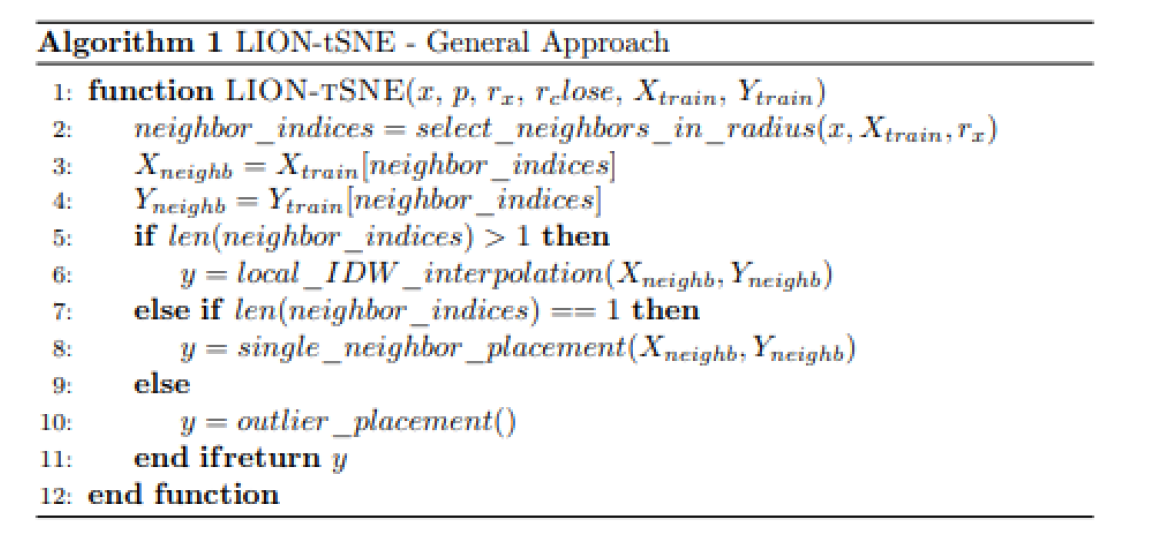
\includegraphics[scale=0.52]{algorithm_lionTSNE_pseudocode.PNG}
\caption{Algorytm tSNE - pseudokod}
\end{figure}

\subsection{LION tSNE - IDW}

Gdy algorytm decyduje, że dany punkt jest inlierem, stosowana jest
technika Inverse Distance Weight Interpolation (IDW). Dla nowego punktu
x jego pozycja F(x) w nowym wymiarze jest wyliczana następująco:

\begin{equation}
    F(x) = \sum_{d(x - x_i) \leq r_x} w_i(x)y_i 
\end{equation}

,gdzie 
$w_i(x) = \frac{d(x - x_j)^{-p}}{\sum_{d(x-x_j) \leq r_x} d(x - x_j)^{-p}}$

$r_x$ - promien odległości dla lokalnego sąsiedztwa w którym jest dodawany
nowy punkt, parametr wywołania

$p$ - parametr wywołania

Zauważmy, że gdy 
$x \rightarrow x_i$ 
to 
$d(x - x_i)^{-p} \rightarrow \infty$
i 
$w_i(x) \rightarrow \infty$ 
i 
$F(x) \rightarrow y_i$

\subsection{LION tSNE - outlier placement}

Główna idea outlier placementu jest nastepujaca: jesli x jest outlierem to
odpowiadająca jej po zmapowaniu wartość y powinna także być
zwizualizowana jako outlier. Aby odnaleźć takie wartości, musimy znaleźć
położenie y, takie że nie ma żadnych sąsiadów w promieniu ry . Promień ry
jest jednym z parametrów algorytmu i jeśli zostanie wybrana zbyt duza
wartość, wtedy z racji na duże odległości między punktami, zmniejsza się
czytelność wykresu natomiast jesli promien zostanie wybrany zbyt mały
klastry i wartości odstające mogą być nierozróżnialne. Dlatego też wartość
ry może być wyznaczona na podstawie pewnego percentylu rozkładu
odległości najbliższych sąsiadów w przestrzeni y (np. 95-ty lub 99-ty
percentyl).

\section{kNN sampling}
\label{sec:kNN}

\subsection{kNN sampling w LION tSNE}

Autorzy artykułu zasugerowali, że sposób próbkowania danych zastosowany
w tSNE jest niewystarczający chociażby przy dynamicznie zmieniających się
danych. Jednocześnie przedstawili kilka kroków potrzebnych do
zrealizowania idei k-NN samplingu.
\begin{enumerate}
    \item Czyszczenie danych za pomocą eliminacji redundantnych punktów i
zainicjalizowanie pustych zmiennych odpowiednimi wartościami.
\item
 Dobór właściwego zbioru treningowego poprzez k-NN sampling.
 \item
 Rzutowanie zbioru treningowego na nisko wymiarowa przestrzeń oraz
dodanie nowych punktów do modelu tSNE.
 \item
 Dla nowych danych interpolacja ich do istniejącego modelu za pomocą
LION-tSNE
 \item
 Wyliczenie precyzji k-NN samplingu dla całego zbioru danych.
\end{enumerate}

\subsection{Wybór zbioru treningowego poprzez k-NN sampling}

Zaproponowana idea k-NN samplingu opiera się na wyliczeniu Nearest
Neighbor score (NNscore) oraz Mutual Nearest Neighbor score
(MNNscore). Mamy dany graf skierowany $G = (V, E)$, gdzie krawędź
$E(v1, v2)$ oznacza, ze $v_2$ jest sąsiadem $v_1$, natomiast sąsiedztwo $v_1$
oznaczamy jako $N_v1$. Stopień wychodzący każdego wierzchołka jest równy
k, a stopień wchodzący zalezy od wartosci współczynnika sąsiedztwa innych
wierzchołków. W celu wyznaczenia optymalnego zbioru treningowego
dobieramy odpowiednie k oraz zbiór punktów wejściowych mapujemy na
wierzchołki grafu k-NN.

Wyznaczamy NN score, który odpowiada stopniu wchodzącemu
wierzchołka $x_i$:

\begin{equation}
    NNscore(x_i) = |\{x_j | x_i \in N_x_j \} | \forall_{j \neq i} x_j \in X
\end{equation}

Gdzie X jest zbiorem danych wejściowych a $N_x_j$ sąsiedztwem $x_j$. Następnie
wyliczamy MNNscore, który dla $x_i$ jest równy co najwyżej k:

\begin{equation}
    MNNscore(x_i) = |\{x_j | x_i \in N_x_j \wedge x_i | x_j \in N_x_i  \} | \forall_{j \neq i} x_j \in X
\end{equation}

Ostatecznie dobór punktu $x_i$ jako próbki treningowej oraz jego sąsiedztwo
jest dany jako:

\begin{equation}
    train\_sample = first\_index\{argmax_{x_i \in  X} \{NNscore(x_i)\} \cap \argmax_{x_i \in X} \{MNNscore(x_i)\}\}
\end{equation}

\subsection{Dodanie nowych punktów do modelu tSNE}

W LION-tSNE stosujemy IDW i Outlier Placement. Nowe dane mogą być
dodawane do modelu tSNE na dwa sposoby, na podstawie wyliczonych
parametrów rxNN, ryNN oraz rclose . Wartość rxNN oznacza minimalny
promien zbioru wejściowego, co z pomocą pewnej heurystyki pozwala na
wskazanie czy dany punkt jest wartością właściwą czy odstająca. Parametr
rclose pozwala na zidentyfikowanie próbek odstających powiązanych z
wartościami odstającymi znajdującymi się w modelu tSNE. Natomiast ryNN
wyznacza minimalna odległość pomiędzy punktami ze zbioru wejściowego,
a próbkami odstającymi oraz dla wartości odstających pomiedzy nimi.

\section{Wyniki projektu}
\label{sec:results}
TODO

\section{Wnioski}
\label{sec:conclusions}
TODO

\bibliographystyle{unsrt}  
%\bibliography{references}  %%% Remove comment to use the external .bib file (using bibtex).
%%% and comment out the ``thebibliography'' section.


%%% Comment out this section when you \bibliography{references} is enabled.
\clearpage
\renewcommand\refname{Źródła}
\begin{thebibliography}{1}

\bibitem{paper} 
Bheekya Dharamsotu ; K. Swarupa Rani ; Salman Abdul Moiz ; C. Raghavendra Rao
\newblock Paper: k-NN Sampling for Visualization of Dynamic Data Using LION-tSNE. 
\newblock {\em https://ieeexplore.ieee.org/abstract/document/8990391}

\end{thebibliography}



\end{document}

